\chapter{Analysis and Algorithms}


In order to compare the data from both vehicles and take appropriate action, this chapter demonstrates how a vehicle obtains information about a nearby vehicle and how that information passes from one component to another inside the vehicle.
 
The analyses and procedures used to create this V2V system, as well as the functions needed to program it, will be presented in detail.

\section{Applying laws of motion}
Vehicles are considered as points in a 2D coordinate system as shown in figure \ref{fig:vectors},
they can be connected to the origin point, then vectors laws are applied to them to calculate the distance between these points.
In the rest state, the Cartesian points are known, so applying the distance vector law is possible.
In general, it is rare to use this concept in the project since the main target is to detect distances with variable time during vehicles motion, so motion laws will take the most significant role in the project.
\begin{figure}[h]
    \centering
    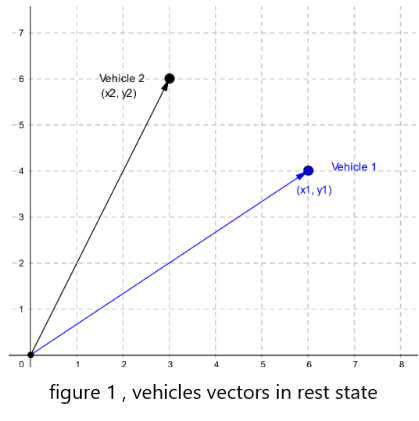
\includegraphics{figure/6_1.png}
    \caption{Vectors of vehicles in rest state}
    \label{fig:vectors}
\end{figure}


To apply motion laws, the project needs to measure the car's velocity and acceleration, but due to 2D coordinate system, the analysis must be done in both x and y components, so not only does the project need linearity information, but also it needs the analysis of x and y components for each peripheral, that is why the project uses  an IMU sensor, a rotary encoder, and a compass; as IMU can extract acceleration components directly ($A_x$, $A_y$, and $A_z$), rotary encoder gives information about linear velocity V, compass gives the angle $\theta$ between the vehicle and north direction, by using the angle and the linear velocity, $V_x$ and $V_y$ can be extracted indirectly by $Vsin(\theta)$ and $V cos(\theta)$ respectively as shown in figure \ref{fig:vx-vy}.
\begin{figure}[h]
    \centering
    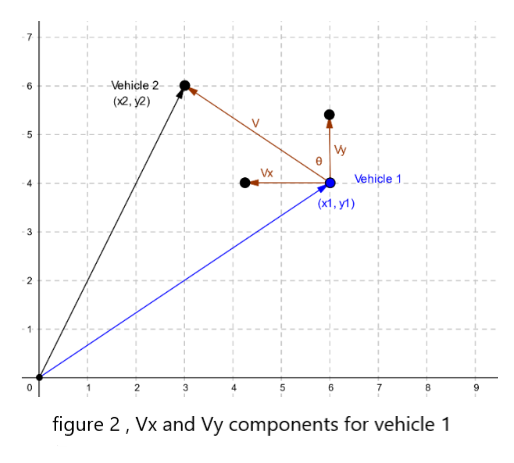
\includegraphics{figure/6_2.png}
    \caption{$V_x$ and $V_y$ components for vehicle 1}
    \label{fig:vx-vy}
\end{figure}
Now, vehicle information is extracted, and motion laws can be applied, the origin point is the intersection between equator and Greenwich calculated using GPS data, next step is to get position of the vehicle relative to the origin point i.e. (x1, y1).

X coordinate represents longitude values and Y coordinate represents latitude values, this data is extracted from GPS module.

\section{Analysis steps}
\begin{enumerate}
    \item Receive neighbor vehicle data from the server to extract longitude, latitude, speed, angle, speed, and acceleration components for neighbor vehicle.
    \item Extract the vehicle data from sensors.
    \item Using the second law of motion with variable time, both $d_x$ and $d_y$ components for both the main vehicle and neighbor vehicle are calculated as shown:
    \[d_x(t) = \frac{1}{2}A_X t^2 + V_x t\]
    \[d_y(t) = \frac{1}{2}A_Y t^2 + V_y t\]
    \item To calculate $d_x$ and $d_y$ for both vehicles, the processor loops over the equations and substitutes t variable with values from 0 to 10 seconds.
    \item In every loop, the processor calculates  \(d_{xvehicle},    d_{yvehicle}\), $d_{xneighbor}$, and $d_{yneighbor}$, then it determines whether $d_{xvehicle} - d_{xneighbor}$ or \(|d_{yvehicle} - d_{yneighbor}\)
equal to zero, if it is true, this means that the two vehicles will be at the same point after time t and collision has occurred, so the processor must send a warning for the user to prevent this future accident immediately.
    \item The previous calculations treat vehicles as if they were points on a plane, however since vehicles have proper dimensions, threshold values, $D_{xmin}$ and $D_{ymin}$  need to be determined based on the actual dimensions of the vehicles.
    \item After that, the main vehicle data is sent to all neighbor vehicles to be processed in other vehicles.
    \item Finally, the processor resets the neighbor variables to be ready to receive other neighbor data and repeat the analysis steps.
\end{enumerate}

\section{Analysis programming code}
This section shows the analysis idea implementation in the programming, and how to write the analysis steps as program codes.

First, there are two definitions that must be taken into consideration; the first one is connection between V2V unit and other neighbor V2V units, and the second one is connection between components inside each V2V.
The first definition is done by connecting all Raspberry Pis inside all V2V units with the server to send and receive JSON files which contain the vehicles data, the code here is written in Python and the implemented functions were:
\begin{itemize}
    \item Send JSON files to multiple clients: data taken from STM needs to be converted to the standard format JSON and sent to the server which is responsible for broadcasting that file to other vehicles.
    \item Receive JSON files from multiple clients: files coming from the server must be received correctly by the Raspberry Pi in the vehicle and sent to the STM to do the previously explained processing.
\end{itemize}
The mechanism in which this happens will be explained thoroughly in the incoming chapters.

The second definition is done by connecting the Raspberry Pi with the STM using UART protocol, and connecting STM with IMU using I2C protocol, GPS module using UART protocol, and rotary encoder using timer peripheral.
After receiving JSON file, Raspberry Pi converts it into string to be sent to STM, and when STM receives it, STM stores it into buffer RX array. Note that both STM and Raspberry Pi  must have the same declaration for transmit “Tx” buffer size and receive “Rx” buffer size, and this value must indicate the maximum size of the sent and received data, and if the data is less than this value, dummy characters are inserted before sending or receiving.

For example, if the sending data size in Raspberry Pi is 30 characters, and the receiving buffer in STM size is 40 characters, the STM will receive the data and wait for another 10 characters to be received, and this causes overlapping between vehicles data.

Another example, if the data sending size in Raspberry Pi  is 30 characters, and the receiving buffer in STM size is 20 characters, the STM will receive only 20 characters and the remaining characters will be lost.
 
- Raspberry Pi implements some functions for JSON file; \textbf{write\_json\_file} and \textbf{read\_json\_file} and this functionality is defined as follows:

\begin{enumerate}
    \item \textbf{write\_json\_file}: to take string from the Raspberry Pi  and extract the vehicle data (neglecting dummy characters) and convert this string into JSON file, JSON file must contain the data values and the IP address of the Raspberry Pi, so it also inserts the IP address into the JSON file.
    \item \textbf{read\_json\_file}: After receiving a JSON file (all JSON files are now containing IP address and vehicle data), this function extracts the vehicle data and converts it into string, and if the size of the string is less than the Tx buffer size, it inserts a dummy char.
    \item \textbf{UART}: This function uses serial library, and it is responsible for calling \textbf{read\_json\_file} and sending it to STM, then receiving string from STM and calling \textbf{write\_json\_file} to convert it into JSON.
    
\end{enumerate}
Inside while (1) in STM, transmission/reception are done, analysis is calculated, data from sensors is extracted. Code in STM is written by C/Embedded C.

\begin{enumerate}
    \item Transmission and reception between STM and Raspberry Pi:
Once the STM receives data from Raspberry Pi by \textbf{HAL\_UART\_Receive\_IT }function and makes the analysis, it generates the TX buffer to send it to Raspberry Pi using \textbf{HAL\_UART\_Transmit} function.
The analysis is done inside \textbf{HAL\_UART\_RxCpltCallback} function to ensure that all reception is done successfully, and all data is inside RX buffer, and after analysis, \textbf{HAL\_UART\_Transmit} is
also called inside \textbf{HAL\_UART\_RxCpltCallback}.
    \item Analysis after receiving:The data into RX buffer is written in the following format:
“longitude,latitude,speed,Ax,Ay,angle,Vx,Vy,Dummy”
Example:
If the received data was: 

“32.123456,29.435213,34.56, +10.21,-3.22,30.567,20.541,17.823, !!!!!”
This means the following:


\bgroup
\def\arraystretch{1.5}% 
\begin{table}[h]
\centering
\begin{tabular}{| c | c |}
\hline
 Longitude &32.123456 \\
 \hline
 Latitude &  29.435213 \\
 \hline
 Speed & 34.56 \\ 
 \hline
 $A_x$ & +10.21  \\
 \hline
 $A_y$ & -3.22  \\
 \hline
 Angle & 30.567  \\
 \hline
 $V_x$ & 20.541 \\
 \hline
 $V_y$ & 17.823 \\
 \hline
 Dummy Data & !!!!!  \\
 \hline

\end{tabular}
\end{table}
\egroup

\end{enumerate}

The analysis is done by implementing some functions, these functions are:

\begin{enumerate}
    \item \textbf{resetBuffersIndexes}: First, this function is called to ensure that the RX and TX buffers indexes point to the first char inside them.
    \item \textbf{splitData}: It takes some data part (this part may define longitude, latitude,..etc) from the RX buffer and convert it into float number and return it.
    \item \textbf{getNeighborData}: It sets the pointer of the RX buffer which detects some data, then it calls \textbf{splitData}() to get the float number and store it into its specific value, then it repeats setting the RX buffer pointer to get all the peripherals values.
    \item \textbf{getCarData}: It connects with sensor drivers and takes the car data from them.
    \item \textbf{sendWarning}: It is responsible for sending the suitable warning message by inserting the message into the Tx Buffer to be sent with vehicle data.
    \item \textbf{analysis}: It is responsible for applying second motion law over variable time (looping over the time) and compare dx components with $D_{X\_min}$ and $d_y$ components with $D_{Y\_min}$, and if there is a danger, it calls the function \textbf{sendWarning}.
    \item \textbf{mergeData}: It takes a float data (this data may define longitude, latitude,..etc) and convert it into string, then it stores it into TX buffer.
    \item \textbf{generateTransmitBuffer}: This function is responsible for generating the specific format “longitude,latitude,speed,Ax,Ay,angle,Vx,Vy,Dummy” , it calls \textbf{mergeData} for every peripheral, then it inserts dummy characters if it is needed.
\end{enumerate}
Here is how these functions are utilized to correctly perform the analysis:
\begin{itemize}
    \item STM calls the \textbf{HAL\_UART\_Receive\_IT} for receiving neighbor vehicle data into Rx buffer, and when is reception is done, HAL driver calls \textbf{HAL\_UART\_RxCpltCallback} automatically, so that all code is written inside this function to ensure that all neighbor data is inside Rx buffer.
    \item The first function will be called in \textbf{HAL\_UART\_RxCpltCallback} is                  \textbf{resetBuffersIndexes} for initializing the indexes of the buffers to point for the first address in both buffers.
    \item After that, \textbf{getNeighborData} is called to get the neighbor vehicle data from RX buffer and convert it into float numbers and store each value into its specific variable.
    \item Next, \textbf{getCarData} is called to get the main vehicle data from the sensors, it is better to call \textbf{getCarData} after \textbf{getNeighborData} and before analysis since the sensors change variables simultaneously and analysis needs the latest updated values for the peripherals.
    \item After that, \textbf{analysis} is called to apply motion laws and detect any future collision.
    \item Next, \textbf{generateTransmitBuffer} is called to insert the main vehicle data into the Tx buffer. Note that the Tx buffer may also contain a warning message.
    \item Finally, using \textbf{HAL\_UART\_Transmit} is called to transmit both data and warning message (if exists) to Raspberry Pi.
\end{itemize}
Now, the Raspberry Pi receives three kinds of data; warning message, vehicle data, and dummy data. Thus, after receiving is done, Raspberry Pi detects the warning message and displays it on its screen, removes dummy data, and converts the vehicle data into JSON file by \textbf{write\_json\_file} function.



